% ============================================================
% SKELETON for the implementation paper (Prompt 15), T21 Version A.
% Same layout as the mid-semester review (article, two-column, natbib).
% Red [WRITE: ...] boxes = notes for YOU to turn into your own sentences.
% Orange [TO VERIFY: ...] = facts to check before submission.
% Every number below comes from results/results.csv (run of 17 Nov 2026).
% Tables in tables/ are written by src/analyse_a.py: never retype numbers.
% Write the Abstract LAST. Delete all \writeit and \tv before submission.
% ============================================================
\documentclass[10pt,twocolumn]{article}

\usepackage[a4paper,margin=1.9cm,columnsep=0.6cm]{geometry}
\usepackage{times}
\usepackage{amsmath}
\usepackage{graphicx}
\usepackage{tikz}
\usetikzlibrary{arrows.meta,positioning}
\usepackage{booktabs}
\usepackage{caption}
\usepackage[colorlinks=true,linkcolor=blue!50!black,citecolor=blue!50!black,urlcolor=blue!50!black]{hyperref}
\usepackage[round]{natbib}
\usepackage{fancyhdr}
\usepackage{titlesec}
\usepackage{enumitem}
\usepackage{xcolor}
\usepackage{abstract}

\setlength{\parindent}{0pt}
\setlength{\parskip}{4pt}
\titleformat{\section}{\normalfont\large\bfseries}{\thesection}{0.6em}{}
\titleformat{\subsection}{\normalfont\normalsize\bfseries}{\thesubsection}{0.6em}{}
\titlespacing*{\section}{0pt}{10pt}{4pt}
\titlespacing*{\subsection}{0pt}{8pt}{3pt}
\pagestyle{fancy}
\fancyhf{}
\fancyhead[L]{\small Verifying LLM Citations: Rules, Strings or Databases?}
\fancyhead[R]{\small AITR Implementation Paper}
\fancyfoot[C]{\small\thepage}
\renewcommand{\headrulewidth}{0.4pt}
\captionsetup{font=small,labelfont=bf}

\newcommand{\writeit}[1]{\textcolor{red!70!black}{\textbf{[WRITE:} #1\textbf{]}}}
\newcommand{\tv}[1]{\textcolor{orange!80!black}{\textbf{[TO VERIFY:} #1\textbf{]}}}

\title{\vspace{-1.2cm}\textbf{Rules, Strings or Databases? Checking Fabricated Citations from Two Open-Weight Language Models}}
\author{Vaibhav Sharma \\ \small Roll No. MSE2026010 \\ \small Department of Software and Automation \\ \small Indian Institute of Information Technology Allahabad (IIIT-A)}
\date{}

\begin{document}
\twocolumn[
  \begin{@twocolumnfalse}
    \maketitle
    \begin{abstract}
    \writeit{Write LAST, 150 to 200 words. Cover in order: the problem (LLMs invent references; checkers are rarely compared on the same data); what you did (2 open-weight 7B models, 6 topics, 108 citations; three checkers B0, B1, B2 against reference labels); the key numbers (95.4\% of citations fabricated; B2 AUC 0.817 vs B1 0.672 vs B0 0.415; B0 recall 0.029; B2 5.18 s and 3.69 API calls per citation); the main caveat (AI-made reference labels sharing sources with B2; 5 real works only); one sentence on what it means.}
    \end{abstract}
    \vspace{0.5em}
  \end{@twocolumnfalse}
]

% ------------------------------------------------------------
\section{Introduction}
\writeit{Four short paragraphs, your words.
(1) Problem: LLMs produce references that look real but do not exist; cite \citet{walters2023} and \citet{alkaissi2023} for early evidence, \citet{ji2023} for hallucination in general.
(2) Gap: many audits report fabrication rates, but the checkers they rely on (format rules, string classifiers, database lookup) are rarely compared on the same citations, with cost; \citet{naser2026} proposes string-only detection, \citet{rao2026} database-based checking \tv{confirm what rao2026 checks}.
(3) What you did: two open-weight models, a frozen protocol, three checkers, two research questions (RQ2 transfer, RQ3 comparison).
(4) Contributions as a bullet list: a measured comparison with cost; a failure analysis of database matching on generic titles; an honest negative result for rule checks and for transfer; a public, reproducible pipeline.
Do not claim novelty of method: this is a comparison study (Prompt 12).}

% ------------------------------------------------------------
\section{Related Work}
\subsection{How often language models fabricate references}
\writeit{Summarise, in your words, the audits: \citet{walters2023} (ChatGPT, bibliographic errors), \citet{linardon2025} (topic familiarity and prompt specificity), \citet{mugaanyi2024} (cross-disciplinary reliability), legal domain \citet{dahl2024} and \citet{magesh2025}, large-scale \citet{xu2026} and \citet{algaba2024}. Point: rates differ widely by model, domain and prompt. Do not copy any percentage you have not re-checked in the original paper (decision D03).}
\subsection{Ways to check a citation}
\writeit{Three families, each with one or two citations: format and consistency checks; string-only learned detectors \citep{naser2026}; database lookup against scholarly indexes \citep{rao2026}; plus self-consistency methods such as \citet{manakul2023} that do not use databases. Say which family each of your B0, B1, B2 belongs to.}
\subsection{Gap}
\writeit{One paragraph: no study you found compares all three on the same open-weight model output with reference labels and cost. Keep it modest: "in the literature reviewed for this work".}

% ------------------------------------------------------------
\section{Method}
\begin{figure}[t]
\centering
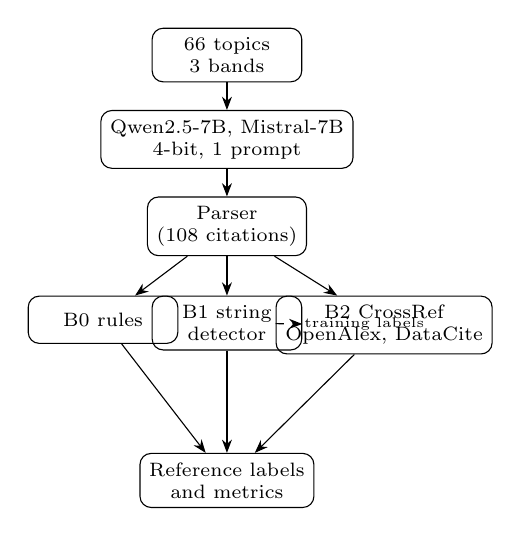
\begin{tikzpicture}[node distance=0.35cm, every node/.style={draw, rounded corners, font=\scriptsize, align=center, minimum width=1.9cm, minimum height=0.6cm}, >=Stealth]
\node (t) {66 topics\\3 bands};
\node (g) [below=of t] {Qwen2.5-7B, Mistral-7B\\4-bit, 1 prompt};
\node (p) [below=of g] {Parser\\(108 citations)};
\node (b0) [below left=0.5cm and -0.4cm of p] {B0 rules};
\node (b1) [below=0.5cm of p] {B1 string\\detector};
\node (b2) [below right=0.5cm and -0.4cm of p] {B2 CrossRef\\OpenAlex, DataCite};
\node (r) [below=1.3cm of b1] {Reference labels\\and metrics};
\draw[->] (t) -- (g); \draw[->] (g) -- (p);
\draw[->] (p) -- (b0); \draw[->] (p) -- (b1); \draw[->] (p) -- (b2);
\draw[->] (b0) -- (r); \draw[->] (b1) -- (r); \draw[->] (b2) -- (r);
\draw[->, dashed] (b2) -- node[draw=none, right, font=\tiny]{training labels} (b1);
\end{tikzpicture}
\caption{Pipeline. B1 is trained on B2 labels and evaluated against reference labels.}
\label{fig:pipeline}
\end{figure}

\subsection{Topics and generation}
\writeit{Facts to describe: 90 candidate computer-science topics; prominence = OpenAlex keyword-search work count \tv{cite OpenAlex once verified}; terciles high/medium/low; 2 pilot topics per band for tuning only; main run used 2 topics per band (decision D25, time limit). Models Qwen2.5-7B-Instruct and Mistral-7B-Instruct-v0.3 \tv{cite tech reports once verified}, 4-bit NF4, revisions pinned (give the two hashes in the appendix or repo). One prompt asking for 10 references with authors, year, title, venue, DOI. Temperature 0.7, top-p 0.9, 1024 new tokens, seed 11.}
\subsection{Parsing}
\writeit{Deterministic regex parser, no LLM; numbered items only; labelled-field reader. Mention the two bugs found in the pilot and fixed before the main run (debugging log 6 and 7) in one sentence: it shows the pipeline was checked against real output.}
\subsection{The three checkers}
\writeit{B0: six red flags from the citation text (no DOI, malformed DOI, no year, implausible year, no authors, title under four words); fabricated if at least 1 flag (D21b, chosen on the pilot).
B1: logistic regression on 16 string features (list them in a short table or footnote); no database feature allowed; trained on B2 labels; evaluated out-of-fold with folds grouped by topic.
B2: query CrossRef (title + first author) and OpenAlex (title); best title similarity (token sort ratio); fabricated if below t = 0.85 (chosen on 57 pilot citations); otherwise metadata checks (surname, year within 1, DOI equality, DOI resolution via CrossRef then DataCite) separate "metadata error" from "exists".}
\subsection{Reference labels}
\writeit{Be explicit and honest: labels were made by an AI assistant with web and database lookups, following a written rubric, and reviewed by you (D24, D27); rule for "same work" (D28). State that most labels used the same databases as B2, so B2's scores are an upper bound. This paragraph is required for integrity; do not soften it.}

% ------------------------------------------------------------
\section{Experimental Setup}
\writeit{Hardware: pilot on Colab T4; main run on Kaggle 2 x T4, both models in parallel, 20.4 minutes in total. Software versions (Kaggle: Python 3.13.16, torch 2.11.0, transformers 5.20.2). Protocol frozen 2026-11-17 11:35 UTC before generation. Metrics: precision, recall, F1 and specificity for "fabricated" with Wilson intervals \tv{cite wilson1927 once verified}; AUC; paired topic bootstrap (1,000 resamples, seed 2026) for F1 differences; cost per citation. Comparator fairness: same citations, same labels, thresholds fixed before the main run. A trivial "all fabricated" row is included because of the high base rate.}

% ------------------------------------------------------------
\section{Results}
\subsection{Corpus}
\writeit{12 answers; 7 cut at 1024 tokens (Qwen 3, Mistral 4); 108 citations, all parsed (Qwen 58, Mistral 50); 7 duplicates inside an answer kept (D19).}

\begin{table}[t]
\centering
\small
\setlength{\tabcolsep}{3pt}
\caption{Fabrication rate under two definitions (B2 labels).}
\label{tab:fr}
\begin{tabular}{llllll}
\toprule
model & fr\_exist & CI & fr\_broad & CI broad & n \\
\midrule
Qwen2.5-7B & 0.879 & 0.77 to 0.94 & 1.000 & 0.94 to 1.00 & 58 \\
Mistral-7B & 0.780 & 0.65 to 0.87 & 1.000 & 0.93 to 1.00 & 50 \\
\bottomrule
\end{tabular}
\end{table}

\subsection{How many citations were fabricated}
\writeit{Point to Table~\ref{tab:fr}. Reference labels: 103 of 108 fabricated (95.4\%), 5 real works with errors, none fully correct. Per model: Qwen 0.948 (0.86 to 0.98), Mistral 0.960 (0.87 to 0.99); overlapping intervals, so no model difference. B2's own rates are lower (0.879, 0.780) because of its misses; explain in one sentence.}

\begin{table*}[t]
\centering
\small
\setlength{\tabcolsep}{3pt}
\caption{Verifier comparison against the reference labels (class: fabricated; Wilson 95\% CIs).}
\label{tab:verifiers}
\begin{tabular}{llllllllll}
\toprule
verifier & precision & P 95\% CI & recall & R 95\% CI & f1 & specificity & tp & fp & fn \\
\midrule
B0 rules & 0.750 & 0.30 to 0.95 & 0.029 & 0.01 to 0.08 & 0.056 & 0.800 & 3 & 1 & 100 \\
B1 string detector & 0.968 & 0.91 to 0.99 & 0.893 & 0.82 to 0.94 & 0.929 & 0.400 & 92 & 3 & 11 \\
B2 database & 0.978 & 0.92 to 0.99 & 0.854 & 0.77 to 0.91 & 0.912 & 0.600 & 88 & 2 & 15 \\
B1 without DOI features (ablation) & 0.969 & 0.91 to 0.99 & 0.913 & 0.84 to 0.95 & 0.940 & 0.400 & 94 & 3 & 9 \\
Trivial: all fabricated & 0.954 & 0.90 to 0.98 & 1.000 & 0.96 to 1.00 & 0.976 & 0.000 & 103 & 5 & 0 \\
\bottomrule
\end{tabular}
\end{table*}

\subsection{RQ3: comparing the checkers}
\writeit{Point to Table~\ref{tab:verifiers}. First explain the trivial row: at a 95\% base rate it gets the best F1 (0.976) with specificity 0, so F1 alone cannot rank the checkers. Then AUC: B2 0.817, B1 0.672, B0 0.415. B0 recall 0.029. B2 minus B0 F1 0.856 (0.771 to 0.933); B2 minus B1 -0.017 (-0.118 to 0.098), so no difference can be claimed. Ablation: B1 without DOI features F1 0.940, i.e.\ removing them did not hurt. Specificity rests on only 5 real works.}

\begin{figure}[t]
\centering
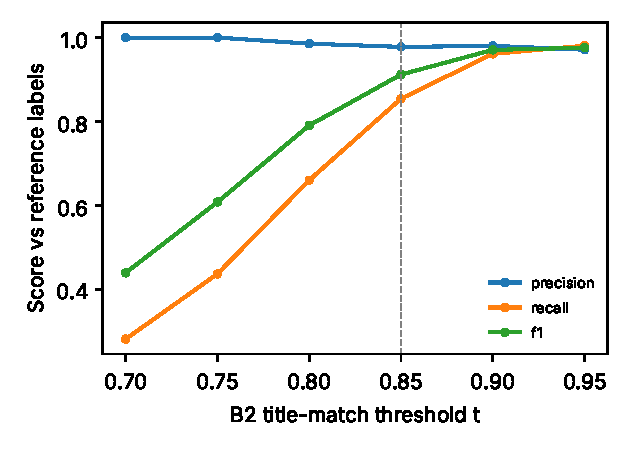
\includegraphics[width=\linewidth]{figures/f2_b2_sensitivity.pdf}
\caption{B2 precision, recall and F1 against the reference labels for title thresholds 0.70 to 0.95 (main run). Dashed line: frozen threshold 0.85.}
\label{fig:sens}
\end{figure}

\subsection{Where database matching fails}
\writeit{17 disagreements (results/b2\_disagreements.csv): 15 invented generic titles scored at or above 0.85 against real papers by other authors (give one example); 2 real papers with altered titles scored below 0.85. Use Figure~\ref{fig:sens}: a higher threshold would catch more fabrications on this data, but that threshold was not chosen in advance, so report it as an observation only.}

\begin{table}[t]
\centering
\small
\setlength{\tabcolsep}{3pt}
\caption{Cost per citation (B1 time includes training within cross-validation).}
\label{tab:cost}
\begin{tabular}{lll}
\toprule
verifier & sec\_per\_cit & api\_per\_cit \\
\midrule
B0 rules & 0.000 & 0.000 \\
B1 string detector & 0.001 & 0.000 \\
B2 database & 5.181 & 3.685 \\
\bottomrule
\end{tabular}
\end{table}

\subsection{Cost}
\writeit{Point to Table~\ref{tab:cost}: B2 5.18 s and 3.69 API calls per citation; B0 and B1 under a millisecond. Mention the CrossRef limit of 3 requests per second (D09) as a reason for B2's speed.}

\begin{table*}[t]
\centering
\small
\setlength{\tabcolsep}{3pt}
\caption{Transfer of the string-only detector B1 (AUC against B2 labels; 95\% topic bootstrap CI of the drop).}
\label{tab:transfer}
\begin{tabular}{llllllll}
\toprule
test\_model & train\_model & auc\_within & auc\_transfer & drop & ci\_lo & ci\_hi & n \\
\midrule
Qwen2.5-7B & Mistral-7B & 0.471 & 0.695 & -0.224 & -0.518 & -0.020 & 58 \\
Mistral-7B & Qwen2.5-7B & 0.371 & 0.408 & -0.037 & -0.241 & 0.262 & 50 \\
\bottomrule
\end{tabular}
\end{table*}

\begin{figure}[t]
\centering
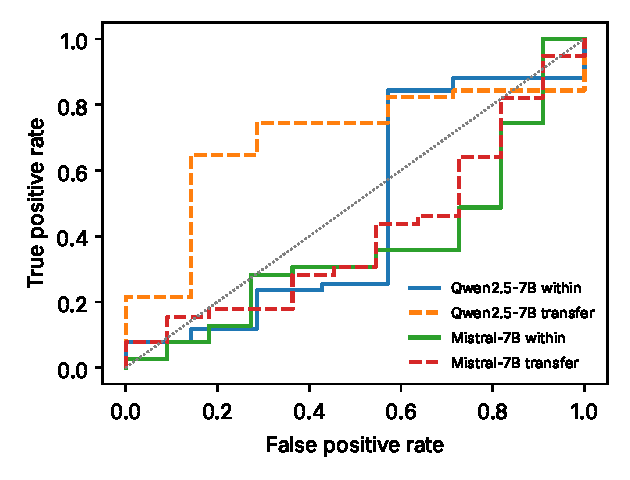
\includegraphics[width=\linewidth]{figures/f1_roc_transfer.pdf}
\caption{ROC curves of B1 within each model and after training on the other model (scored against B2 labels).}
\label{fig:roc}
\end{figure}
\subsection{RQ2: does the string detector transfer?}
\writeit{Point to Table~\ref{tab:transfer} and Figure~\ref{fig:roc}. Within-model AUC below 0.5 for both models (0.471, 0.371): B1 did not learn within one model, with only 18 non-fabricated B2 labels over 6 topics. Transfer AUC 0.695 and 0.408. The planned decision rule (drop above 0.05 with CI excluding 0, D06) cannot be applied meaningfully; report RQ2 as inconclusive.}

% ------------------------------------------------------------
\section{Discussion}
\writeit{Use the Prompt 14 outline, section by section: supported (database beats rules), unresolved (string detector vs database), contradicted (rules as a cheap filter for these models), not testable (transfer). Give mechanisms as possibilities, not facts: well-formed fabrications defeat format rules; generic titles defeat title similarity. One paragraph on what a practitioner can take away, kept within your data.}

\section{Limitations}
\writeit{In this order: (1) AI-made reference labels sharing sources with B2; (2) 6 topics, 108 citations, 5 real works, one seed, one run; (3) 7 of 12 answers truncated; (4) two 7B models in 4-bit, one prompt, no commercial or agentic tools despite the topic title; (5) protocol changes before freezing (D08, D25); (6) pilot and main on different platforms.}

\section{Future Work}
\writeit{The three ranked follow-ups from Prompt 14: human relabelling of 47 citations with kappa; an author-aware B2 for generic titles; a full 60-topic run with 2048 tokens.}

\section{Conclusion}
\writeit{Four to five sentences: what was compared, the two clearest findings (rules fail; database matching is best by AUC but misses generic titles), the main caveat, the public pipeline.}

\section*{AI Assistance Disclosure}
\writeit{Required by Section 10 of the brief. State: code was written with an AI assistant and tested by you; you ran the pilot (Colab) and main run (Kaggle); the reference labels were AI-made and reviewed by you; the paper text is yours. Point to ai\_assistance\_log.md and research\_decisions.md in the repository.}

\section*{Code and Data Availability}
\writeit{GitHub URL \tv{add after Prompt 17}. Everything needed to reproduce the tables: configs/protocol\_v1.yaml, data/, results/results.csv, notebooks/.}

\bibliographystyle{plainnat}
\bibliography{refs}

\end{document}
